\chapter{Programmable Logic Controllers (PLCs)}
\begin{quotation}
    \noindent\textsf{ The diffusion of more and more powerful and cheap computer has given the possibility to introduce in the field of industrial automation \textit{Programmable Logic Controllers (PLCs). Such devices, with respect to traditional technologies, bring with them a lot of advantages. After a brief introduction about the different tipologies of traditional hardware for industrial automation, we will focus our attention on PLCs of which we present features and programming modalities.}}
\end{quotation}
\minitoc

\begin{figure}[h]
    \centering
    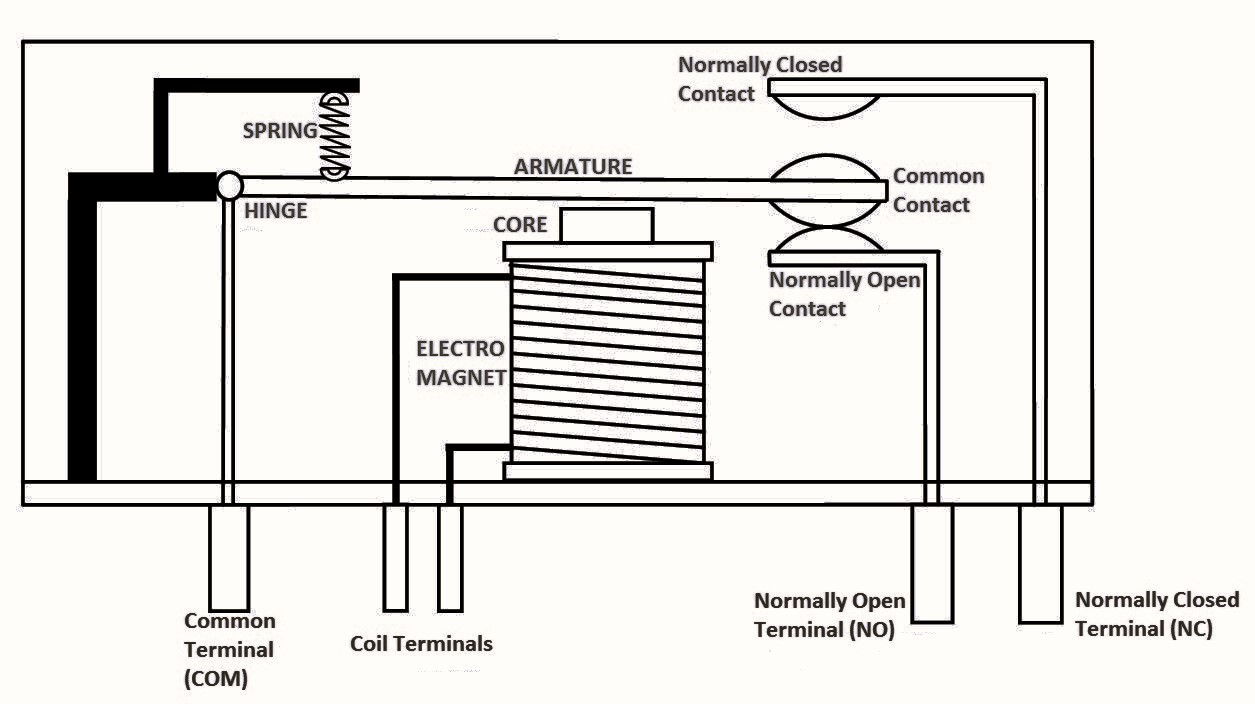
\includegraphics[scale=0.4]{img/relay_scheme.jpg}
    \caption{Relay scheme }    
\end{figure}
\vspace{-0.5cm}
\section{Industrial Automation Hardware}
In the field of \textit{Industrial automation} the controllere can be found at different places: (i) directly in the senso or in the actuator (analog PIDs), as a separate device or as an algorithm in a computer (here there is the possibility to manage a great number of loops). There are many possibilities to realize a controller: 
\begin{description}
    \itemsep-0.3em
    \item[Wired relay systems] At first in absence of computers and programmable devices, controllers was realized through \textit{\textbf{relays}}\footnote{
        A \textbf{relay} is a simple electromechanical device that use a magnetic field to control a switch. In this device there is a coil that, when energized creates a magnetic field that pushing a piece of metal close/open the switch.
    } and dedicated control loops; the number of such devices for automating the production was not negligible: you can imagine that the changeover time was not short at all, too. The schematic given by the engineers to the electricians which embeds the logic to implement was called \textit{ladder schematic} which used to display sensors, motors, valves, relays you were able to find into the system. Such systems were based on mechanical systems whose moveable parts represented a problem to face. Moreover, if only one relay stopped working, the entire system had to be checked.
    \item[Analog circuits] A step forward was made introducing \textit{operational amplifier} in order to implement PID controllers; there are several circuits exploiting the \textit{virtual ground principle} in order to simulate the proportional, integrative and derivative blocks.   
    \item[Embedded circuits] More modern technologies which are \textit{microprocessor-based}. They are designed for a specific task and are parts of more complex systems including other hardware and mechanical parts. They have a lot of advantages, among the other: low power consumption and reduced sizes. They can be based on microcrocontroollers, DSP, microprocessors or FPGAs.
    \item[Industrial PC] It is nothing but a PC integrated with specific expansions, machine interfaces, expanded communication ports and so on. They are characterized by different construction properties which make them more suitable to the context they are used in (for example: alternative cooling methoeds, heavier metal for the external frame...)
    \item[PLCs] (Programmable Logic Controllers) whose main features are well-explained in the next paragraphs. 
\end{description}

\section{The advent of PLCs}
The realization of low cost computer made possible the most recent evolution in automatin industrial plants: the advent of PLCs. This phenomena begain in 70s. More specifically, in 1968 \textit{General Motors} issued a first PLC prototype request in order to progressively substitute hard-wired relays.
\begin{definition}
    A \textbf{PLC} is a real-time microprocessor-based system that implement functions as   \textit{logic, sequencing, timing} and \textit{arithmetic operations} in order to perform some control tasks.
\end{definition}

PLCs, probably, will remain predominant on the factory floor. This is due to some particular features:
\begin{itemize}
    \itemsep-0.3em
    \item They can be used to control complex mutlivariable systems; 
    \item They are reprogrammable, for this reason they can be reapplied to different systems; 
    \item The fact a computational abitily can be used, they can address even more complicated control tasks.
    \item They have analog and digital I/Os with standard levels. Depending on the tipology they can have a large number of peripherals.
    \item They are relatively cheap, while the value is the in the application software.
\end{itemize}

\begin{figure}
    \centering
    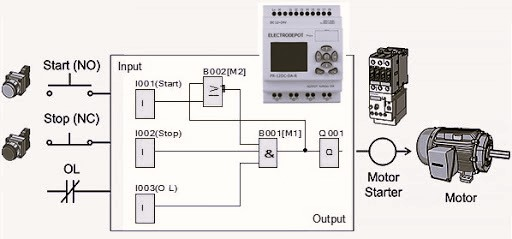
\includegraphics[scale=0.7]{img/PLC_scheme.jpg}
    \caption{An example schematic for a PLC}
\end{figure}

The first PLCs were programmmed using the same schematic used for describing the realization of wired relay-based systems (ladder diagrams). This eliminated the need to teach the technicians to program them. Nowadays, ladder diagrams are the most common way to program a PLC. \\
It is remarkable, that there is a standard, the IEC 61131-3, which enumerates five programming languages for PLCs which are splittable into two categories: (i) \textbf{graphical languages} which comprises Function Block Diagram (FBD), Ladder Diagram (LD) and Sequential Flow Chart (SFC); (ii) \textbf{textual languages} which comprises Instruction List and Structured text.

\subsection{PLC connections}
How the PLCs is used? When a process is controlled by using a PLC it uses input from sensors to make decisions and provides outputs which drives actuators. The control loop, as usual, is continuous cycle for: (i) reading the  inputs, (ii) solving the ladder logic, (iii) changing the outputs accordingly.

\section{Ladder diagrams}  
How we mentioned before, \textbf{ladder logic} is the main programming method for PLCs that mimic the relay logic and it has been explained why the decision to use it was a strategic one\footnote{Note that nowadays relays are also used in modern control systems but not for implementing the logic which is almost totally demanded to PLCs}.
An example of ladder schematic is given in the \Cref{fig:ladder}.

\begin{figure}[h]
    \centering
    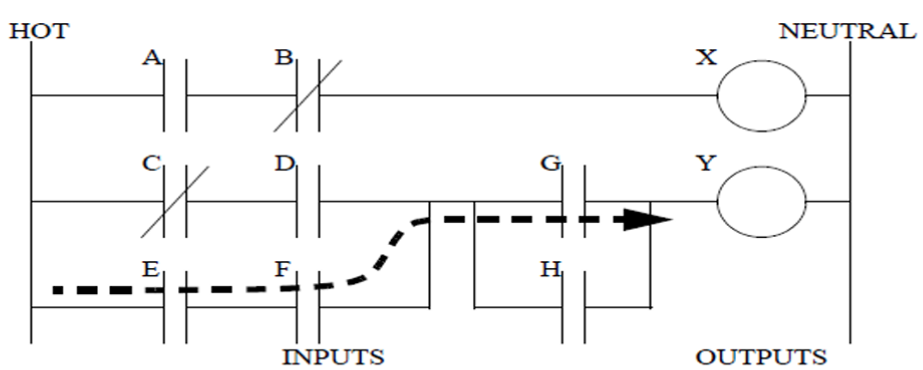
\includegraphics[scale=0.5]{img/sample.png}
    \caption{Example of ladder schematic}
    \label{fig:ladder}
\end{figure}

Just to give a bit of terminology, the power flows from left to  right among two rails which are called \textbf{hot} and \textbf{neutral} rails. A basic element of a ladder schematic is the \textbf{rung} which in which there are combinations of \textit{inputs} (vertical lines, barred vertical lines) and \textit{outputs} (circles). An input can come from a sensor, while the \textit{output} is some device which is external from the controller (light, motors) which is switched on or switched off.

\subsection{Ladder logic Inputs}
There are tipically two types of inputs for the ladder schematic: \textit{normally open} and \textit{normally closed} inputs. In the former case, an active $x$ will  close the contact and allow power to flow; in the latter case, power flows into the input whether the input $x$ is not closed. 

\begin{figure}
    \centering
    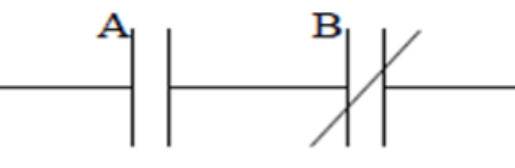
\includegraphics[scale=0.5]{img/ladder_inputs.png}
    \caption{\textit{Normally open} and \textit{normally closed} inputs}
\end{figure}

\subsection{Ladder logic Outputs}
In general, in ladder logic, there multiple types of output, but not always they are supported from all PLCs. The most common one is represented by a circle, this type of output when energized will turn on (normal output). There are also more complicate types of output which allows us to latch an output value until we do not decide to unlatch it. 

\begin{figure}[h]
    \centering
    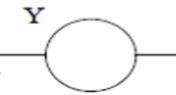
\includegraphics[scale=1]{img/ladder_output.png}
    \caption{\textit{Normal output} ladder symbol}
\end{figure}

\subsection{Example: Design of an alarm for an house}
\begin{remark}
    There is a strong correspondence between boolean logic and ladder schematics. In particular, one from the problem can obtain a suitable boolean function, which being simplified\footnote{
    Using some method. For example: Boolean algebra theorems or Karnaugh maps.
    } can be realized through a ladder schematic. Namely, in the following there are the schematics for the AND and OR ports. The NOT is realized through a \textit{normally closed} input. 
\end{remark}



\begin{figure}[h]
    \centering
    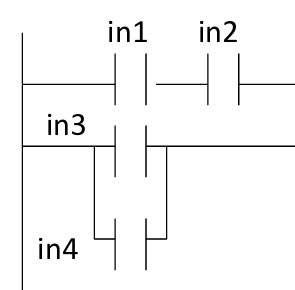
\includegraphics[scale=0.7]{img/and_or.png}
    \caption{AND and OR schematics. The series of two normally open switch can be used to model an AND, the parallel connection between two normally open inputs realize an OR.}
\end{figure}

\noindent
Now, we want to obtain the ladder schematic which solves the following problem:
\begin{quotation}\textsf{\noindent
        Consider the design of a burglar alarm for a house. When activated an alarm and lights will be activated to encourage the unwanted guest to leave. This alarm will be activated if an unauthorized intruder is detected by window sensor and a motion detector. The window sensor os effectively a piece of thin metal which encircles the window. If the window is broken, the foil breaks breaking the conductor (normally closed switch). The motion sensor is designed so that when a person is detected the output will go on. An activate/deactivate switch is also needed.}
\end{quotation}
\noindent
The basic operation of the alarm system is summarized in the following. In particular, the \textit{inputs and outputs} of the system are chosen to be:
\begin{quotation}
    \noindent
    A=Alarm and lights switch (1=on)\\
    W=Window/Door sensor (1=OK)\\
    M=Motion Sensor (0=OK)\\
    S=Alarm Active switch (1=on)
\end{quotation}
The basic operation of the alarm can be described by the following rules:
\begin{quotation}\vspace{-0.5cm}\noindent
    \begin{itemize}
        \itemsep-0.3em
        \item If alarm is on, check sensors.
        \item Is window/door is broken (turns off), sound alarm and turn on lights.
    \end{itemize}
\end{quotation}
The next step is building a \textbf{truth table} summarizing the behaviour of the alarm system. Using some simplification technique (Boolean algebra or Karnaugh maps) the simplified boolean expression related to truth table is:
\begin{equation}
    A=S\cdot{(\bar{W}+M)}
\end{equation}
which in ladder logic can be realized by using the series between $S$ and the parallel $(\bar{W}+M)$.   

\begin{figure}
    \centering
    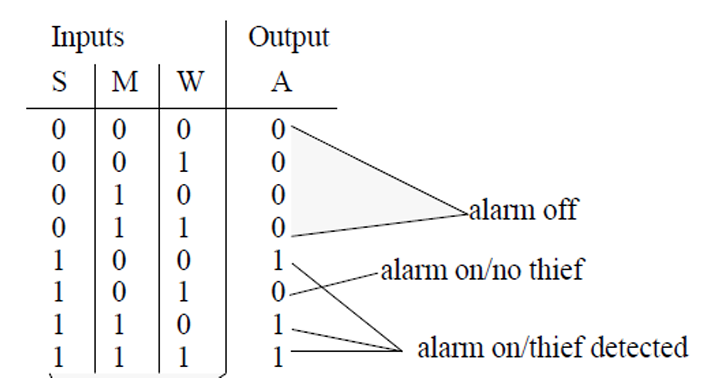
\includegraphics[scale=0.6]{img/example_truth_table.png}
    \caption{Truth table for the \textit{Burglar Alarm} example}
\end{figure}

\begin{figure}
    \centering
    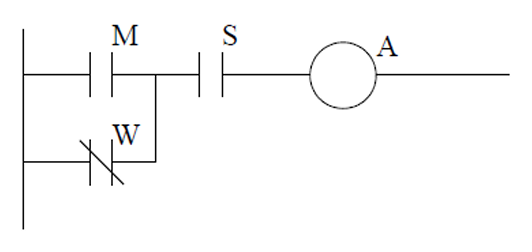
\includegraphics[scale=0.7]{img/example_burglar_ladder.png}
    \caption{Ladder schematic for the \textit{Burglar Alarm} example}
\end{figure}

\subsection{Latches, Counters, Timers}
Till now we have seen the basic building block to obtain any combinatorial function we want. More complex systems cannot be controlled with the combinatorial part alone. Typical, more sophisticated operations one would to solve are: (i) block a certain output and properly unlock it; (ii) waiting that a certain time elapses; (iii) count some events.

\subsubsection{Latches}
A \textbf{latch} is like a \textit{sticky switch}: when you push it down it will turn on, but after it stick in place, it must be pulled in order to turn it off. In ladder logic for a single latch there are two symbols one for latch the output (a circle with a L), another for unlatching it (a circle with a U). 
\begin{remark}
    If an output \textbf{has been latched on} it will keep its valu, even if the power has been turned off.
\end{remark} 

\begin{figure}[h]
    \centering
    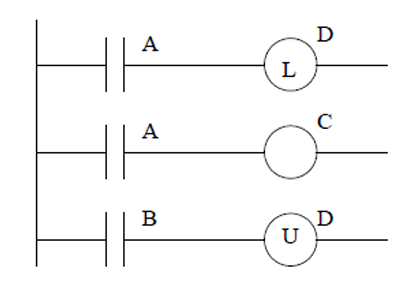
\includegraphics[scale=0.7]{img/latches.png}
    \caption{Schematic for latch/unlatch the output}
\end{figure}
In order to better understand how such devices work, we propose a \textit{timing diagram} with inputs A, B and outputs C, D. It is interesting to observe that while C is on only when A is on, the output D is instead locked (latched) until the input B is not active, this event automatically turns off the output D.

\begin{figure}[h]
    \centering
    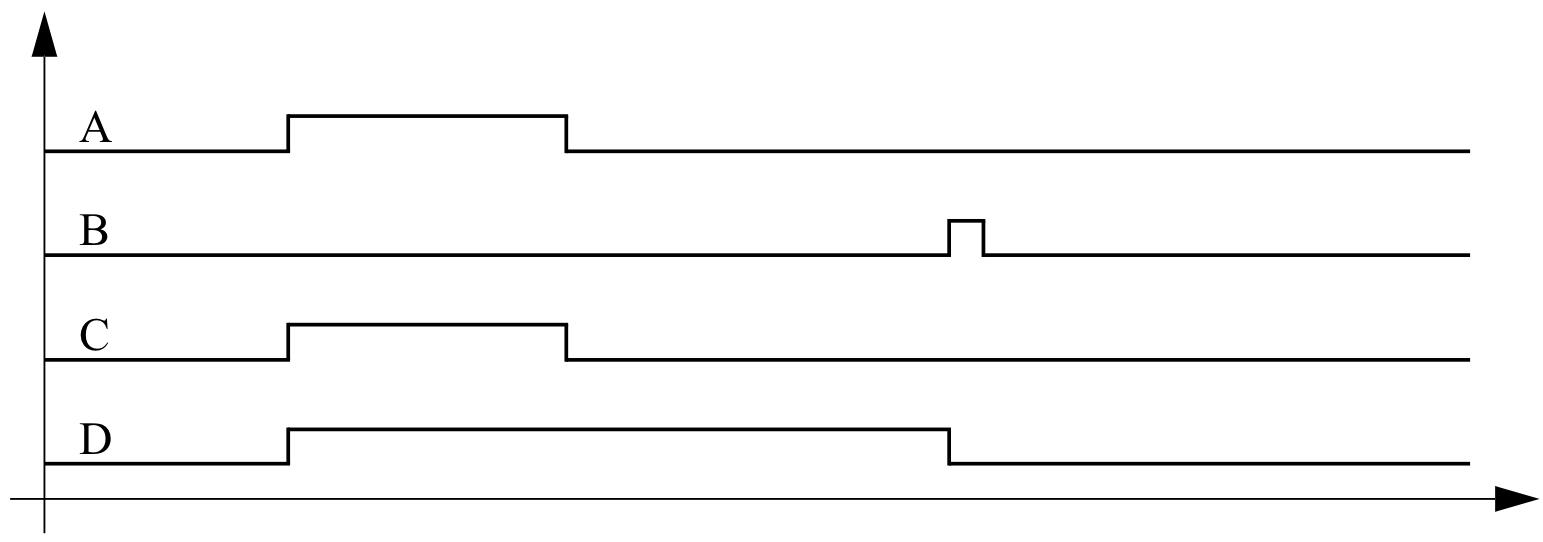
\includegraphics[scale=0.25]{img/timing_latched.jpeg}
    \caption{Timing diagram}
\end{figure}

Such devices have different behaviour with respect to latches, with the only difference that for them a different notation is used.

\subsubsection{Timers}
There are tipically two types of timers: 
\begin{enumerate}
    \itemsep-0.3em
    \item \textit{On-delay timers} whose output is \underline{activated} after a certain time interval elapses; 
    \item \textit{Off-delay timers} whose output is \underline{deactivated} after a certain time interval elapses.
\end{enumerate}

Here we consider only \textbf{non-retaining timers}, when they are turned off, the time delay starts from zero. In the following we give the typical representation for a sample timer. 

\begin{figure}
    \centering
    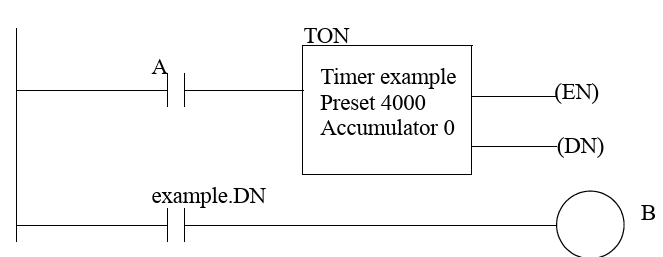
\includegraphics[scale=0.7]{img/ladder_timers.png}
    \caption{Ladder schematic for a timer}
    \label{fig:timeron}
\end{figure}

The one showed in \Cref{fig:timeron} activates and starts incrementing the \textit{Accumulator} when $A$ is activated. The (EN) output is active whenever $A$ is active while the output (DN) is active when incrementing \textit{Accumulator} the value in \textit{Preset} is reached. In the specific case, when the timer elapses the output $B$ will be activated, and will be active until $A$ will be active. \\
To be more precise and clear, look at \Cref{fig:timing_timer}. After 3s the signal A is active for other 3s. Such a time is not sufficient to reach the Preset value (here we assume that the step is 1000ms, that is a 1 is added to the Accumulator each 1000ms). Since we are treating here a \textit{(non-retaining) on-delay timer}, when A deactivate, Accumulator immediately goes to 0. Let us observe now the interval $[9,13]$, here 5 seconds elapses, such interval is sufficient to reach Preset and for activating the output (EN). 
\begin{remark}
    Note that an auxiliary input \texttt{example.DN} is used in order to activate the output B, when the time interval elapses.
\end{remark}

\begin{figure}
    \centering
    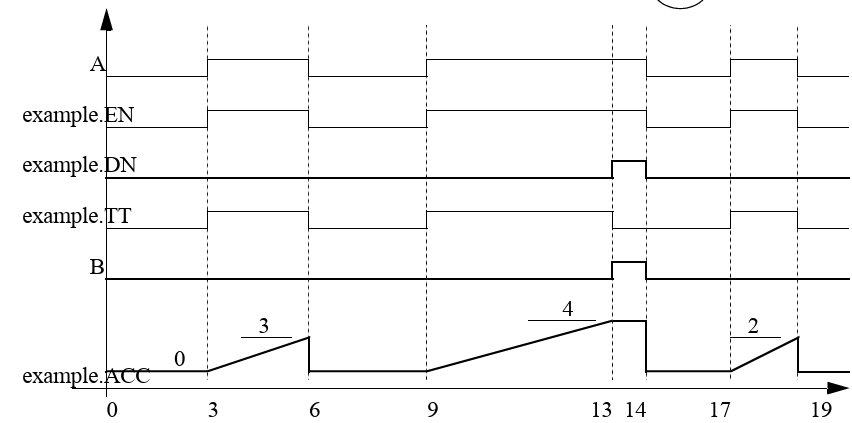
\includegraphics[scale=0.8]{img/timer_example.png}
    \caption{Timing diagram for the timers}
    \label{fig:timing_timer}
\end{figure}

\subsubsection{Counters}
There are two types of counters: \textit{count-up} and \textit{count-down} one. The first when the input signal is active increment of a unit an Accumulator whatever is its duration\footnote{
    Note that this is the same to state that counters (whatever its type is) is sensitive to the LOW-UP variation.
}.

\begin{figure}
    \centering
    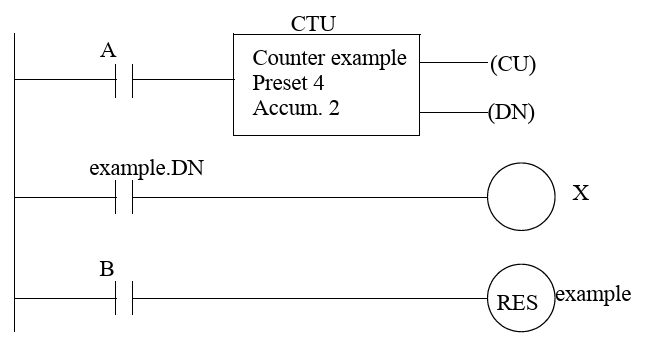
\includegraphics[scale=0.7]{img/CTU_ladder_counter.png}
    \caption{Example of \textit{Count-up counter}}
    \label{fig:CTU}
\end{figure}

Similarly than before, when the value of the Accumulator will reach the Preset value, (DN) will be activated. A counter-down, whether the input A is active decrement the accumulator of one unit. The timer showed in \Cref{fig:CTU} is a count-up counter whose with value of Preset and Accumulator equal to, respectively, 4 and 2. The output X will be active once the auxiliary input \texttt{example.DN} is active. On the other hand, when B will be active the Accumulator will be reset to 0.

\subsubsection{Internal Bits}
When dealing with simple program, (real) inputs can be used in order to set, (real) ouptut. When the situation becomes much harder, programs can use \textbf{memory locations} that are neither inputs nor outputs. These are also referred as \textit{internal relays} or \textit{control relays}. In modern PLCs they can be defined as \textit{variables} of type BOOL. They are very useful in order to implement complex programs.

